\documentclass[10pt,landscape,a4paper]{article}
%\usepackage[utf8]{inputenc}
%\usepackage[ngerman]{babel}
\usepackage[normalem]{ulem}
\usepackage{tikz}
\usetikzlibrary{shapes,positioning,arrows,fit,calc,graphs,graphs.standard}
\usepackage[nosf]{kpfonts}
\usepackage[t1]{sourcesanspro}
%\usepackage[lf]{MyriadPro}
%\usepackage[lf,minionint]{MinionPro}
\usepackage{bold-extra}
\usepackage{multicol}
\usepackage{wrapfig}
\usepackage[top=0mm,bottom=1mm,left=0mm,right=1mm]{geometry}
\usepackage[framemethod=tikz]{mdframed}
\usepackage{microtype}
%\usepackage{physics}
\usepackage{tabularx}
\usepackage{hhline}
\usepackage{makecell}
\usepackage{mathtools}

\usepackage{listings}

\DeclarePairedDelimiter{\ceil}{\lceil}{\rceil}

\newcommand\codeblue[1]{\textcolor{blue}{\code{#1}}}

\usepackage{lastpage}
\usepackage{datetime}
\yyyymmdddate
\renewcommand{\dateseparator}{-}
\let\bar\overline

\definecolor{myblue}{cmyk}{1,.72,0,.38}

\def\firstcircle{(0,0) circle (1.5cm)}
\def\secondcircle{(0:2cm) circle (1.5cm)}

\colorlet{circle edge}{myblue}
\colorlet{circle area}{myblue!5}

\tikzset{filled/.style={fill=circle area, draw=circle edge, thick},
outline/.style={draw=circle edge, thick}}

\pgfdeclarelayer{background}
\pgfsetlayers{background,main}

%\everymath\expandafter{\the\everymath \color{myblue}}
%\everydisplay\expandafter{\the\everydisplay \color{myblue}}

\everymath\expandafter{\the\everymath\scriptstyle}

\renewcommand{\baselinestretch}{.8}
\pagestyle{empty}

\global\mdfdefinestyle{header}{%
  linecolor=gray,linewidth=1pt,%
  leftmargin=0mm,rightmargin=0mm,skipbelow=0mm,skipabove=0mm,
}

\newcommand{\header}{
  \begin{mdframed}[style=header]
    \footnotesize
    \sffamily
    CS3210 Finals Cheatsheet v1.1 (\today)\\
    by~Julius Putra Tanu Setiaji,~page~\thepage~of~\pageref{LastPage}
  \end{mdframed}
}

\let\counterwithout\relax
\let\counterwithin\relax
\usepackage{chngcntr}

\usepackage{verbatim}

\usepackage{etoolbox}
\makeatletter
\preto{\@verbatim}{\topsep=0pt \partopsep=0pt }
\makeatother

\counterwithin*{equation}{section}
\counterwithin*{equation}{subsection}
\usepackage{enumitem}
\newlist{legal}{enumerate}{10}
\setlist[legal]{label*=\arabic*.,leftmargin=2.5mm}
\setlist[itemize]{leftmargin=3mm}
\setlist[enumerate]{leftmargin=3.5mm}
\setlist{nosep}
\usepackage{minted}

\def\code#1{\texttt{#1}}

\newenvironment{descitemize} % a mixture of description and itemize
{\begin{description}[leftmargin=*,before=\let\makelabel\descitemlabel]}
{\end{description}}

\newcommand{\descitemlabel}[1]{%
  \textbullet\ \textbf{#1}%
}
\makeatletter



\renewcommand{\section}{\@startsection{section}{1}{0mm}%
  {.1ex}%
  {.1ex}%x
{\color{myblue}\sffamily\scriptsize\bfseries}}
\renewcommand{\subsection}{\@startsection{subsection}{1}{0mm}%
  {.1ex}%
  {.1ex}%x
{\sffamily\bfseries}}
\renewcommand{\subsubsection}{\@startsection{subsubsection}{1}{0mm}%
  {.1ex}%
  {.1ex}%x
{\rmfamily\bfseries}}



\def\multi@column@out{%
  \ifnum\outputpenalty <-\@M
    \speci@ls \else
  \ifvoid\colbreak@box\else
    \mult@info\@ne{Re-adding forced
    break(s) for splitting}%
    \setbox\@cclv\vbox{%
      \unvbox\colbreak@box
    \penalty-\@Mv\unvbox\@cclv}%
  \fi
  \splittopskip\topskip
  \splitmaxdepth\maxdepth
  \dimen@\@colroom
  \divide\skip\footins\col@number
  \ifvoid\footins \else
    \leave@mult@footins
  \fi
  \let\ifshr@kingsaved\ifshr@king
    \ifvbox \@kludgeins
      \advance \dimen@ -\ht\@kludgeins
      \ifdim \wd\@kludgeins>\z@
        \shr@nkingtrue
      \fi
    \fi
    \process@cols\mult@gfirstbox{%
      %%%%% START CHANGE
      \ifnum\count@=\numexpr\mult@rightbox+2\relax
        \setbox\count@\vsplit\@cclv to \dimexpr \dimen@-1cm\relax
        \setbox\count@\vbox to \dimen@{\vbox to 1cm{\header}\unvbox\count@\vss}%
      \else
        \setbox\count@\vsplit\@cclv to \dimen@
      \fi
      %%%%% END CHANGE
      \set@keptmarks
      \setbox\count@
      \vbox to\dimen@
      {\unvbox\count@
        \remove@discardable@items
    \ifshr@nking\vfill\fi}%
    }%
    \setbox\mult@rightbox
    \vsplit\@cclv to\dimen@
    \set@keptmarks
    \setbox\mult@rightbox\vbox to\dimen@
    {\unvbox\mult@rightbox
      \remove@discardable@items
  \ifshr@nking\vfill\fi}%
    \let\ifshr@king\ifshr@kingsaved
  \ifvoid\@cclv \else
    \unvbox\@cclv
    \ifnum\outputpenalty=\@M
  \else
    \penalty\outputpenalty
  \fi
  \ifvoid\footins\else
    \PackageWarning{multicol}%
    {I moved some lines to
      the next page.\MessageBreak
      Footnotes on page
    \thepage\space might be wrong}%
  \fi
  \ifnum \c@tracingmulticols>\thr@@
\hrule\allowbreak \fi
  \fi
  \ifx\@empty\kept@firstmark
    \let\firstmark\kept@topmark
    \let\botmark\kept@topmark
  \else
    \let\firstmark\kept@firstmark
    \let\botmark\kept@botmark
  \fi
  \let\topmark\kept@topmark
  \mult@info\tw@
  {Use kept top mark:\MessageBreak
    \meaning\kept@topmark
    \MessageBreak
    Use kept first mark:\MessageBreak
    \meaning\kept@firstmark
    \MessageBreak
    Use kept bot mark:\MessageBreak
    \meaning\kept@botmark
    \MessageBreak
    Produce first mark:\MessageBreak
    \meaning\firstmark
    \MessageBreak
    Produce bot mark:\MessageBreak
    \meaning\botmark
  \@gobbletwo}%
  \setbox\@cclv\vbox{\unvbox\partial@page
  \page@sofar}%
  \@makecol\@outputpage
  \global\let\kept@topmark\botmark
  \global\let\kept@firstmark\@empty
  \global\let\kept@botmark\@empty
  \mult@info\tw@
  {(Re)Init top mark:\MessageBreak
    \meaning\kept@topmark
  \@gobbletwo}%
  \global\@colroom\@colht
  \global \@mparbottom \z@
  \process@deferreds
\@whilesw\if@fcolmade\fi{\@outputpage
    \global\@colroom\@colht
  \process@deferreds}%
  \mult@info\@ne
  {Colroom:\MessageBreak
    \the\@colht\space
    after float space removed
  = \the\@colroom \@gobble}%
  \set@mult@vsize \global
  \fi}
  \global\let\tikz@ensure@dollar@catcode=\relax

  \def\mathcolor#1#{\@mathcolor{#1}}
  \def\@mathcolor#1#2#3{%
    \protect\leavevmode
    \begingroup
    \color#1{#2}#3%
    \endgroup
  }

  \makeatother
  \setlength{\parindent}{0pt}

  \setminted{tabsize=2, breaklines}
  % Remove belowskip of minted
  \setlength\partopsep{-\topsep}


  \newcolumntype{a}{>{\hsize=1.5\hsize}X}
  \newcolumntype{b}{>{\hsize=.25\hsize}X}

  \setlength\columnsep{1.5pt}
  \setlength\columnseprule{0.1pt}
  
  \DeclareMathSizes{5}{5}{5}{5} 
\begin{document}
\setlength{\abovedisplayskip}{0pt}
\setlength{\belowdisplayskip}{0pt}

\tiny
\begin{multicols*}{4}
  \raggedcolumns
  \section{Processes, Threads, and Synchronisation}
  \subsection{Processes \& Threads: abstractions of flow of control}
  \subsubsection{Processes}
  \begin{itemize}
    \item Identified by PID, Own address space, exclusive access to its data, Requires explicit comm for inter-process info exchange, Context switching between processes, must save state, overhead.
    \item 2 types of exec: time slicing (pseudo-parallelism), parallel exec of procs on diff resources
    \item Create new process: \texttt{fork} or \texttt{exec(char *prog, char *argv)}
  \end{itemize}
  \textbf{Disadvantages}: Creating a new process is costly (syscall overhead, all data structures must be allocated, initialised, copied), IPC is costly (must go through the OS)
  \subsubsection{Threads}
  \begin{itemize}
    \item Share the address space of the process -- all threads belonging to the same process see the same value -> \textbf{shared-memory arch}
    \item Thread generation is faster than process generation, diff threads can be assigned to run on diff cores of a multicore.
    \item 2 types:
          \begin{itemize}
            \item \textbf{User-level threads}: managed by a thread lib -- OS unaware of user-level threads. \textbf{Advantages:} switching thread context is fast, \textbf{Disadvantages:} OS cannot map diff threads of same process to diff exec resources -> no parallelism, OS cannot switch to another thread is 1 thread execs a blocking I/O op
            \item \textbf{Kernel threads}: OS is aware of existence.
          \end{itemize}
    \item Global vars and all dynamically allocated data objects can be accessed by any thread
    \item Each thread has a private stack for function stack frames, existing iff the thread is active.
    \item No of threads shld be suitable to parallelism deg of application, available exec resources, not too large to keep the overhead small for thread creation, management, termination
  \end{itemize}
  \subsection{Synchronisation}
  \begin{itemize}
    \item \textbf{Race condition} = 2 concurrent threads accessed a shared resource without access sync
    \item Use \textbf{mutual exclusion} to sync access to shared resources, to protect \textbf{critical section} (c.s.)
    \item Requirements:
          \begin{enumerate}
            \item \textbf{Mutual exclusion (mutex)}: if one thread is in the critical section, then no other is
            \item \textbf{Progress}: If some thread T is not in the c.s., then T cannot prevent some other thread S from entering the c.s. A thread in the c.s. will eventually leave it
            \item \textbf{Bounded waiting (no starvation)}: If some thread T is waiting on the critical section, then T will eventually enter the critical section
            \item \textbf{Performance}: The overhead of entering \& exiting the critical section is small w.r.t. the work being done within it.
          \end{enumerate}
    \item \textbf{Starvation}: a process is prevented from making progressing because some other process has the resource it requires.
    \item \textbf{Deadlock} among a set of processes: if every process is waiting for an event that can be caused only by another process in the set. can arise when processes compete for access to limited resources, incorrectly synced.
    \item Condition for deadlock: if and only if these 4 conditions hold simultaneously:
          \begin{enumerate}
            \item \textbf{Mutex}: at least 1 resource must be held in non-sharable mode
            \item \textbf{Hold and wait}: 1 process holding 1 resource and waiting for another resource
            \item \textbf{No preemption} -- Resources cannot be preempted (c.s. cannot be aborted externally)
            \item \textbf{Circular wait} -- There must exist a set of processes $p_1, p_2, ... p_n$ such that $p_1$ is waiting for $p_2$, $p_2$ for $p_3$, so on.
          \end{enumerate}
    \item 4 Mechanisms:
  \end{itemize}
  \begin{enumerate}
    \item \textbf{Locks}
          \begin{itemize}
            \item 2 operations: \texttt{acquire()} to enter c.s., \texttt{release()} to leave c.s.
            \item Pair calls to acquire and release, can spin (\textbf{spinlock}) or block (\textbf{mutex})
          \end{itemize}
    \item \textbf{Semaphores}
          \begin{itemize}
            \item Abtract data type that provide mutex through atomic counters
            \item "Integers" that support 2 operations: \texttt{wait()} -- decrement, block until semaphore is open. \texttt{signal()}, increment, allow another thread to enter
            \item Safety property: semaphore value $\geq 0$
            \item 2 Types: \textbf{Mutex/binary semaphore} -- only 1 can enter c.s., \textbf{Counting/general semaphore} -- multiple can enter c.s.
            \item Drawback: shared global var, no connection b/w semaphore \& data being controlled, used for both c.s. (mutex) and coordination (scheduling), hard to use, bug-prone
          \end{itemize}
    \item \textbf{Monitors \textmd{(the thread is "in the monitor")}}
          \begin{itemize}
            \item Guarantees mutex, only 1 thread can execute any monitor procedure at any time
            \item If 2nd thread invokes a monitor procedure when a 1st thread is alr executing, it blocks (monitor has to have a wait queue)
            \item If a thread within a monitor blocks, another one can enter
            \item Programming lang construct that controls access to shared data, added by compiler, enforced at runtime
            \item Encapsulates: Shared data structure, procedures that operate on the shared data structures, sync b/w concurrent threads that invoke the procedures
          \end{itemize}
    \item \textbf{Condition Variables}
          \begin{itemize}
            \item Support 3 operations: \texttt{wait()} -- release monitor lock, wait for condition var to be signalled, \texttt{signal()} wake up one waiting thread, \texttt{broadcast} wake up all waiting threads
          \end{itemize}
    \item \textbf{Barrier}
    \item \textbf{Messages}\\
          Simple model of communication \& sync based on atomic transfer of data across a channel
  \end{enumerate}
  \subsubsection{Classical Synchronisation Problems}
  Producer-consumer (finite, infinite buffer), Readers-writers, dining philosophers, barbershop
  \begin{enumerate}
    \item \textbf{Producer-consumer}
  \end{enumerate}
  \begin{verbatim}
mutex = Semaphore(1)
items = Semaphore(0)

// Producer                           // Consumer
event = waitForEvent()                items.wait()
// finite: spaces.wait()              mutex.wait()
mutex.wait()                          event = buffer.get()
buffer.add(event)                     mutex.signal()
mutex.signal()                        // finite: spaces.signal()
items.signal()                        event.proces()
\end{verbatim}
  \subsection{Implementing Locks}
  \begin{itemize}
    \item Implementation of locks has c.s., therefore impl of acquire/release must be atomic
    \item Req HW support: atomic instruction, disable/enable interrupts (prevents context switches)
    \item \textbf{Test-and-set}: record old value, set value, return old value. Hardware executes atomically
  \end{itemize}
  \begin{minted}{C}
struct lock { int held = 0; }
void acquire(lock) { while(test_and_set(&lock->held)); }
void release(lock) { lock->held = 0; }
  \end{minted}
  \begin{itemize}
    \item \textbf{Problem}: spinlocks are wasteful -- thread spinning on a lock -> thread holding the lock cannot make progress on uniprocessor if lockholder yields/sleeps/involuntary context switch.
  \end{itemize}
  \section{Parallel Computing Platforms -- Arch Memory}
  \begin{itemize}
    \item Recap: $\text{CPU Time} = \frac{\text{Instructions}}{\text{Program}}\times\frac{\text{cycles}}{\text{instruction}}\times\frac{\text{seconds}}{\text{cycle}} = \frac{\text{seconds}}{\text{program}}$
    \item \textbf{Instruction/Program} affected by compiler \& ISA, \textbf{Cycles/Instruction} affected by processor implementation, \textbf{seconds/cycle} affected by clock speed (clock freq)
  \end{itemize}
  \subsection{Sources of processor performance gain: ($x$ parallelism, $x$ is ...)}
  \begin{itemize}
    \item \textbf{Bit level}: word size, larger so no need bitslicing
    \item \textbf{Instruction level}: \textbf{pipelining} (parallelism across time, split instr exec in multiple stages, allow multiple instr to occupy different stages in the same clock cycle given no data/control deps), \textbf{superscalar} (paralellism across space, duplicate pipelines, allow multiple instr to pass through the same stage, dispatching multiple instr to diff exec units in the processor, but scheduling is challenging (deciding which instr can be exec together))
    \item \textbf{Thread level}: processor provides HW support for the thread context -- info specific to each thread (PC, Registers, etc) so software threads can execute in parallel. E.g. SMT: Intel HT
    \item \textbf{Process level} -- process has independent memory space, communicate with IPC through OS. can be mapped to multiple processor cores
    \item \textbf{Processor level}: \textbf{Shared memory}, \textbf{Distributed Memory}
  \end{itemize}
  \subsection{Flynn's Parallel Architecture Taxonomy}
  \textbf{SISD (Single Instruction Single Data)}: Single instruction stream is executed, each instruction work on single data. E.g. uniprocessor; \textbf{SIMD}
  Single instruction stream, working on multiple data, exploting data parallelism, known as vector processor. E.g. SSE, AVX in x86; \textbf{MISD}
  Multiple instruction streams, all instruction work on the same data at any time, no actual impl; \textbf{MIMD} Each PU fetch its own instruction, each PU operates on its data. Most popular model for multiprocessor, \textbf{Variant -- SIMD + MIMD}
  Stream processor (GPU's): a set of threads executing the same code (SIMD), multiple set of threads executing in parallel (MIMD)
  \subsection{Memory Organisation}
  \begin{tabularx}{0.5\columnwidth}{X}
    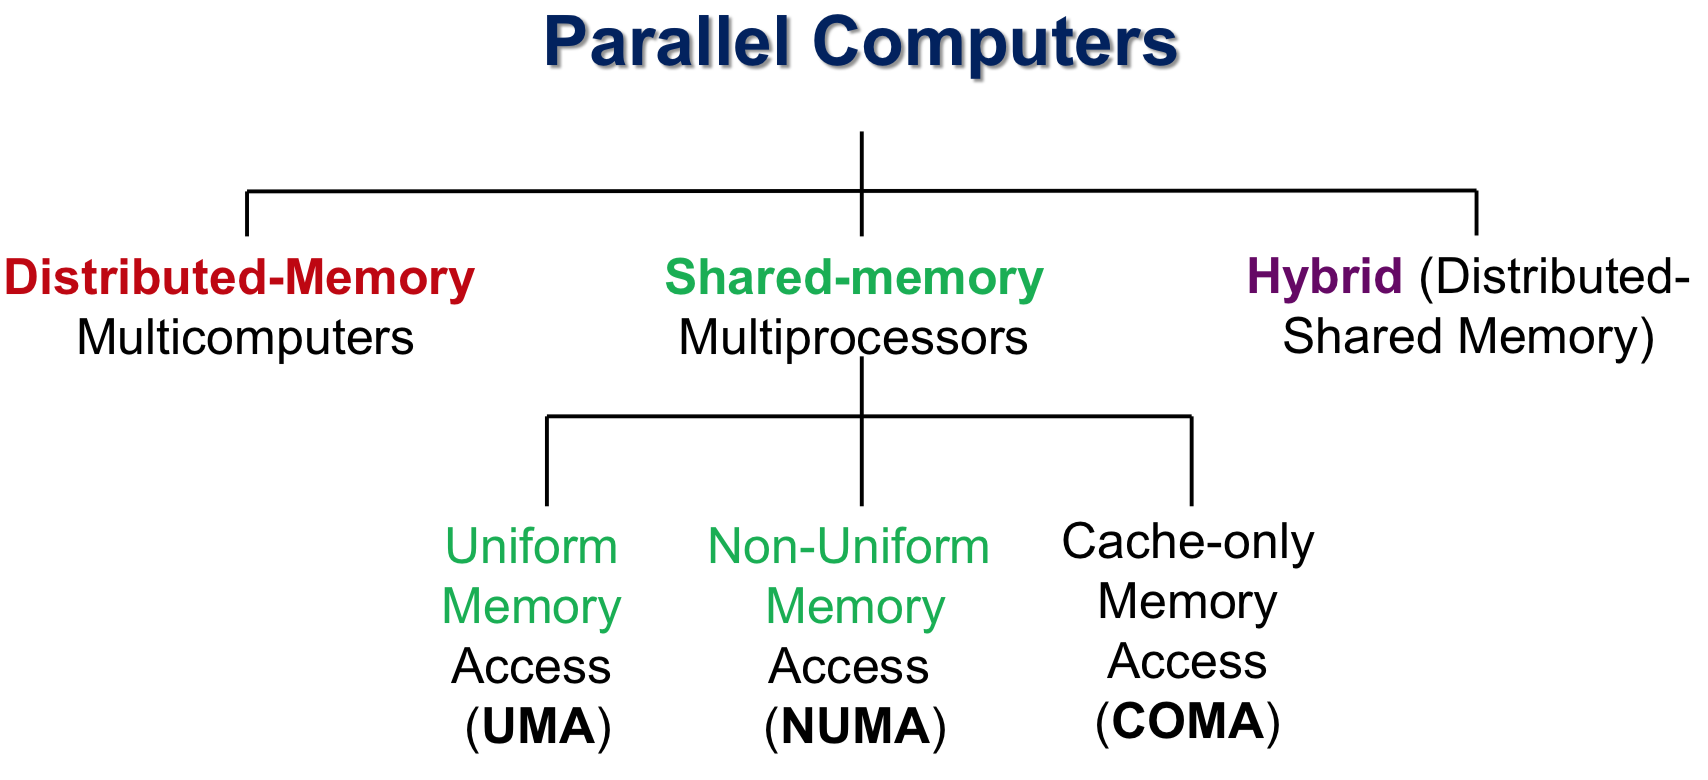
\includegraphics[width=\linewidth]{memory}
  \end{tabularx}
  \begin{tabularx}{0.5\columnwidth}{X}
    \subsubsection{CC (Cache Coherence Protocol)}
    e.g. ccNUMA, each node has cache memory to reduce contention
    \subsubsection{UMA (Uniform Memory Access)}
    Latency of accessing the main mem uniform for all processor, suitable for small no of processors
  \end{tabularx}
  \subsubsection{NUMA (Non-Uniform Memory Access)}
  Diagram just like Distributed-Memory system
  \subsubsection{COMA (Cache Only Memory Architecture)}
  Each memory block works as cache memory, data migrates dynamically and continuously according to the cache coherence scheme
  \begin{itemize}
    \item Physically distributed memory of all processing elements are combined to form a global shared-memory address space, also called distributed shared-memory.
    \item Accessing local mem faster than remote mem for a processor.
  \end{itemize}
  \subsubsection{Distributed-Memory System}
  \vspace{-1mm}
  \begin{tabularx}{0.5\columnwidth}{X}
    \begin{itemize}
      \item Each node is an indep unit with processor, memory and peripheral elements.
      \item Physically distributed memory module: mem in a node is private
      \item Data exchanges between nodes with message-passing
    \end{itemize}
  \end{tabularx}
  \begin{tabularx}{0.5\columnwidth}{X}
    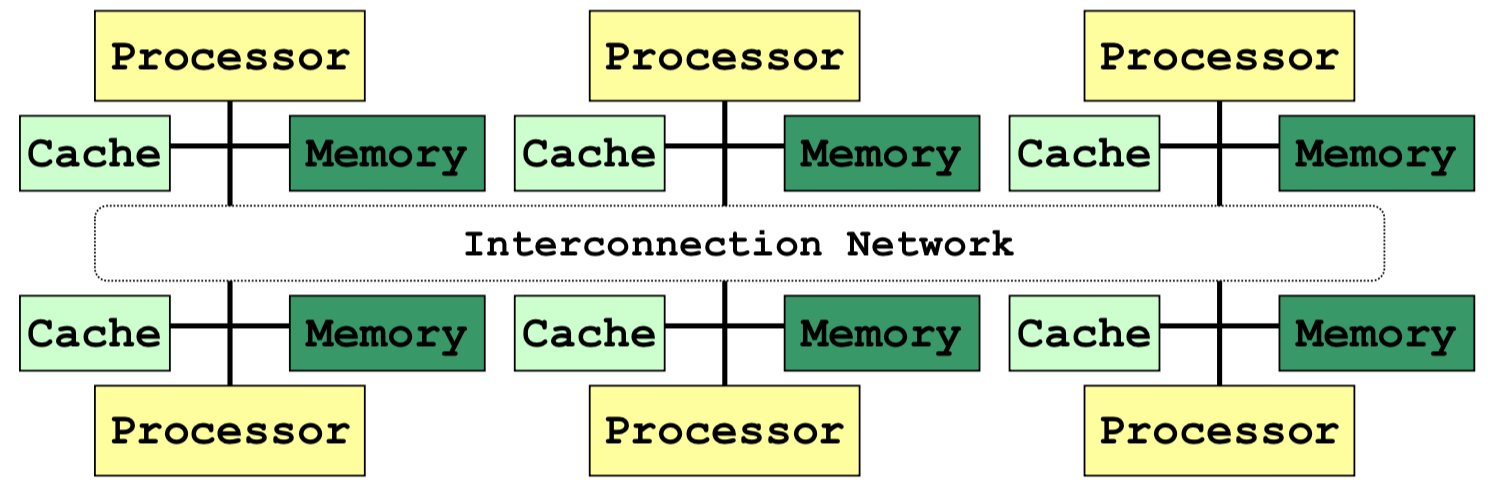
\includegraphics[width=\linewidth]{distributed}
  \end{tabularx}

  \vspace{-1mm}
  \subsubsection{Shared Memory System}
  \vspace{-1mm}
  \begin{tabularx}{0.5\columnwidth}{X}
    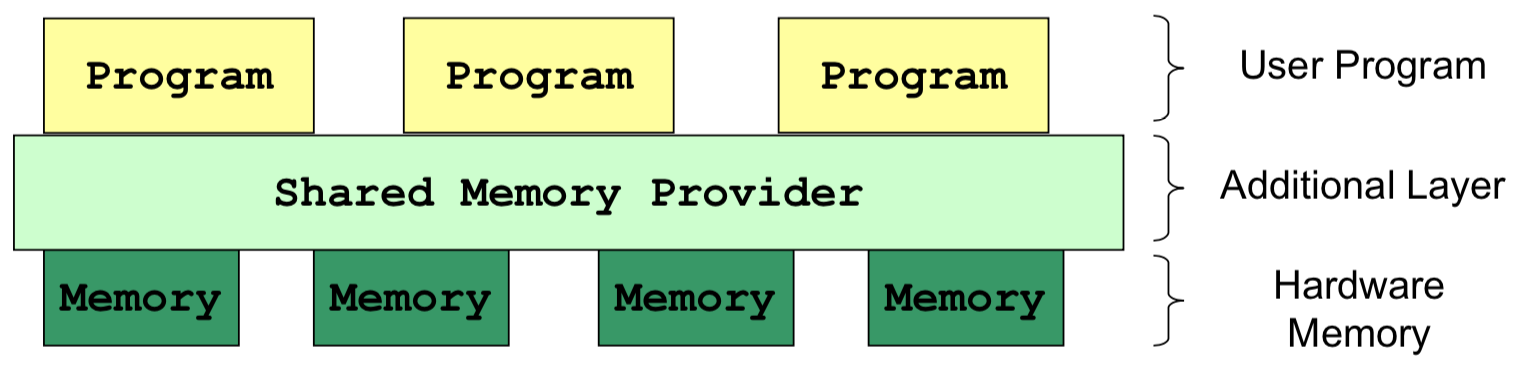
\includegraphics[width=\linewidth]{shared}
  \end{tabularx}
  \begin{tabularx}{0.5\columnwidth}{X}
    \begin{itemize}
      \item Access memory through shared memory provider which maintain the illusion of shared memory.
      \item Program is unaware of the actual hardware memory architecture
    \end{itemize}
  \end{tabularx}
  \vspace{-1.5mm}
  \begin{itemize}
    \item Data exchange between nodes with shared variables
    \item \textbf{Advantages}: no need to partition code/data or physically move data among processors -> communication is efficient
    \item \textbf{Disadvantages}: Special sync constructs are required, lack of scalability due to contention
  \end{itemize}
  \subsubsection{Hybrid (Distributed-Shared Memory)}
  \begin{tabularx}{0.8\columnwidth}{X}
    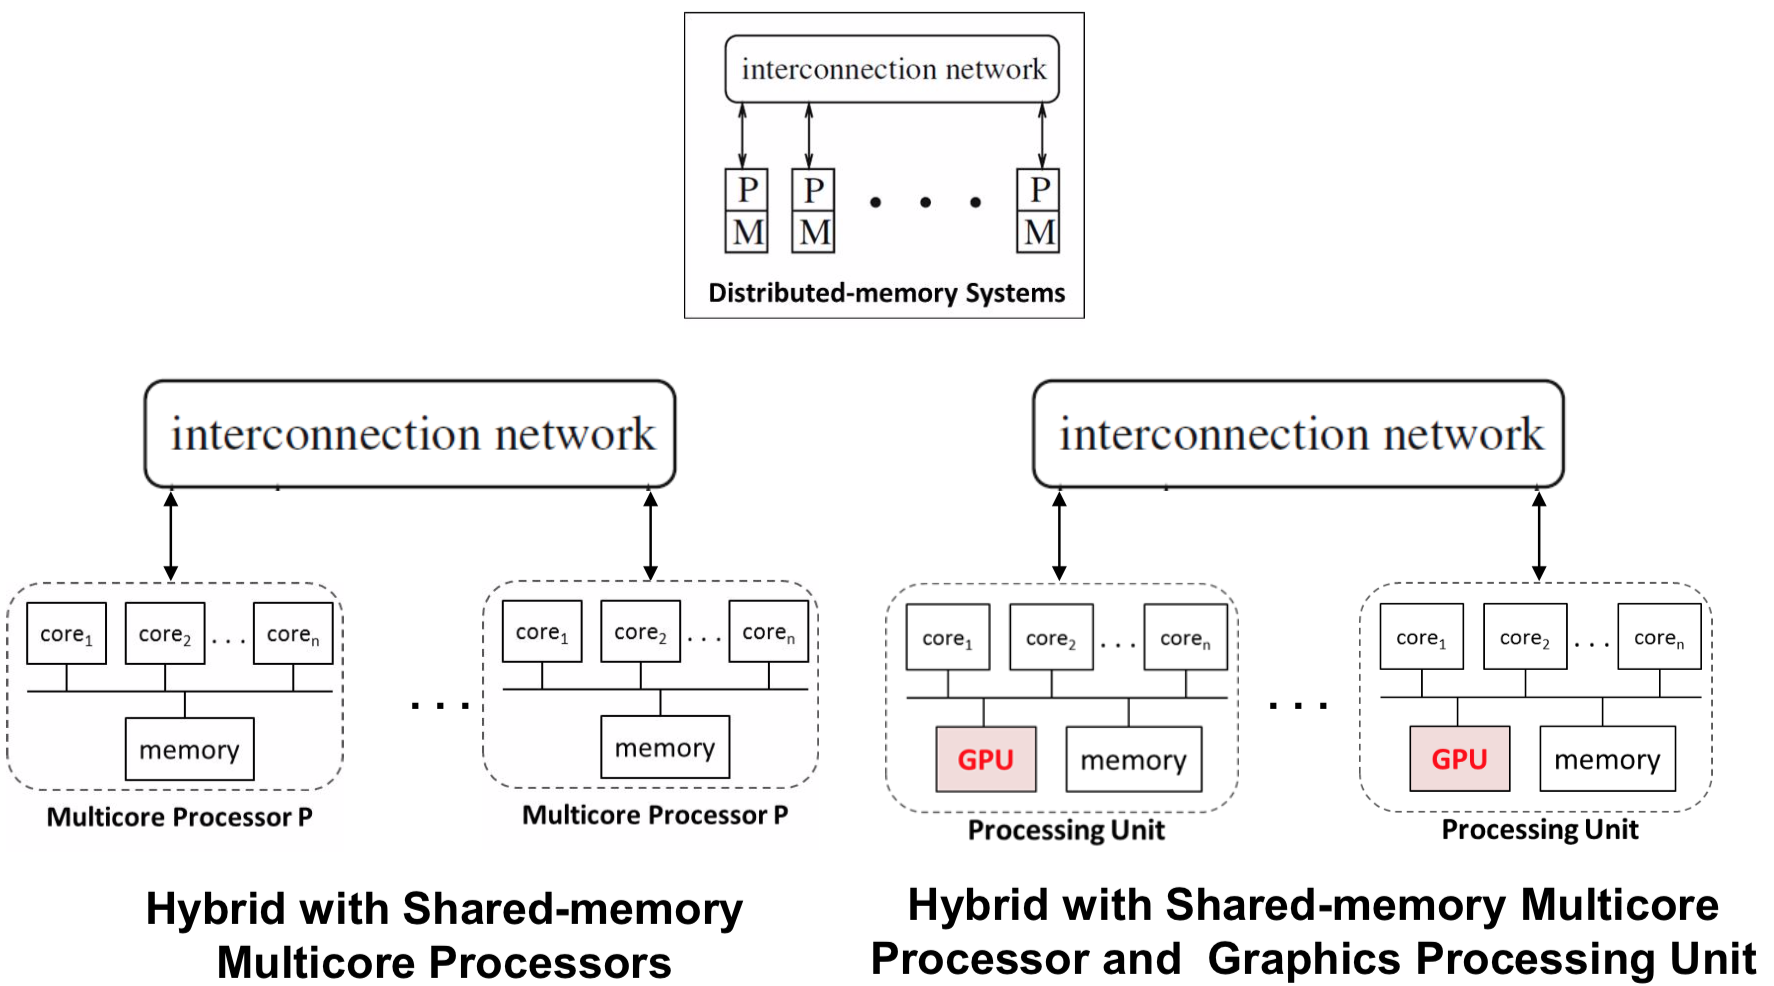
\includegraphics[width=\linewidth]{distributed-shared}
  \end{tabularx}
  \begin{tabularx}{0.18\columnwidth}{X}
    e.g. Hybrid with GPU
  \end{tabularx}
  \subsection{Multicore Architecture}
  \subsubsection{Hierarchical Design}
  \begin{itemize}
    \item Multiple cores share multiple caches, cache size increases from the leaves to the root.
    \item Usages: standard desktop, server processors, GPUs
  \end{itemize}
  \subsubsection{Pipelined Design}
  \begin{itemize}
    \item Data elements processed by multiple exec cores in a \textbf{pipelined} way, from one core to next
    \item Useful if same computation steps have to be applied to a long sequence of data elements, e.g. network processors used in routers and graphic processors
  \end{itemize}
  \subsubsection{Network-based Design}
  \begin{itemize}
    \item Cores and their local caches and memories are connected via an interconnection network
  \end{itemize}
  \section{Parallel Programming Models}
  Common classification:
  \begin{itemize}
    \item \textbf{Level of parallelism}: granulaty from instruction -> statement -> procedural (function/methods) level or parallel loops
    \item \textbf{Specification of parallelism}: implicit/user-defined explicit
    \item \textbf{Execution}: e.g. SIMD/SPMD, sync or async
    \item \textbf{Communication mode}: message-passing/shared vars
    \item \textbf{Synchronisation (coordination mechanisms)}
  \end{itemize}
  \subsection{Decomposition}
  \begin{itemize}
    \item Generate enough tasks to keep all cores busy at all times (no of tasks $\geq$ no of cores)
    \item Granularity is large compared to scheduling \& mapping time (size of task $>>$ overhead of parallelism), \textbf{Static} at program start/compile time, \textbf{Dynamic} during runtime
  \end{itemize}
  \subsection{Scheduling (Static/Dynamic)}
  Find an efficient task exec order to optimise a given objective. Good load balancing among tasks: Computations, Memory accesses (shared), Communication ops (distributed)
  \subsection{Mapping}
  \begin{itemize}
    \item Assignment of processes/threads to execution units
    \item Focuses on perf: Equal utilisation of exec units, minimal comm b/w processors
  \end{itemize}
  \subsection{Parallelism}
  \begin{itemize}
    \item Avg no of units of work that can be perf in parallel/unit time. Work = task + dependencies.
    \item Types in increasing task size: instruction -> loop -> data -> task
  \end{itemize}
  \subsubsection{Instruction Parallelism}
  Multiple instr exec may be inhibited by 3 types of data deps. Data dependency graph
  \begin{itemize}
    \item \textbf{Flow dep (RAW)}/ true dependency: (\textbf{a}) \texttt{a = b + c; e = a + d}
    \item \textbf{Anti-dependency (WAR)}: (\textbf{b}) \texttt{a = b + c; b = d + e;}
    \item \textbf{Output dep (WAW)}: (\textbf{a}) \texttt{a = b + c; a = d + e;}
  \end{itemize}
  \subsubsection{Loop Parallelism}
  If iterations are indep, they can be exec'd in arbitrary order \& in parallel on different processors
  \subsubsection{Data Parallelism}
  \begin{itemize}
    \item \textbf{Partition the data} used in solving the problem among the processing units; each processing unit carries out similar operations on its part of the data
    \item Same op is applied to diff elements of a data set, if ops are independent, elements can be distributed among processors for parallel execution, or using SIMD computers/instructions
    \item e.g. \texttt{for (i = 0; i < N; i++) a[i] = b[i - 1] + c[i];}
    \item On MIMD, common model: SPMD (Single Program Multiple Data) -- 1 parallel program is executed by all processors in parallel (both shared \& distributed address space)
  \end{itemize}
  \subsubsection{Task Parallelism}
  \begin{itemize}
    \item \textbf{Partition tasks} in solving the problem among processing units
  \end{itemize}
  \subsection{Task Dependence Graph}
  \begin{itemize}
    \item DAG, \textbf{node}: task, value = expected exec time; \textbf{edge}: control dep b/w task
    \item \textbf{Properties}:
          \begin{itemize}
            \item \textbf{Critical Path Length}: min (fastest) completion time
            \item \textbf{Degree of concurrency} = total work / critical path length (indication of amount of work that can be done concurrently)
          \end{itemize}
  \end{itemize}
  \subsection{Representation of parallelism}
  \begin{tabularx}{0.5\columnwidth}{X}
    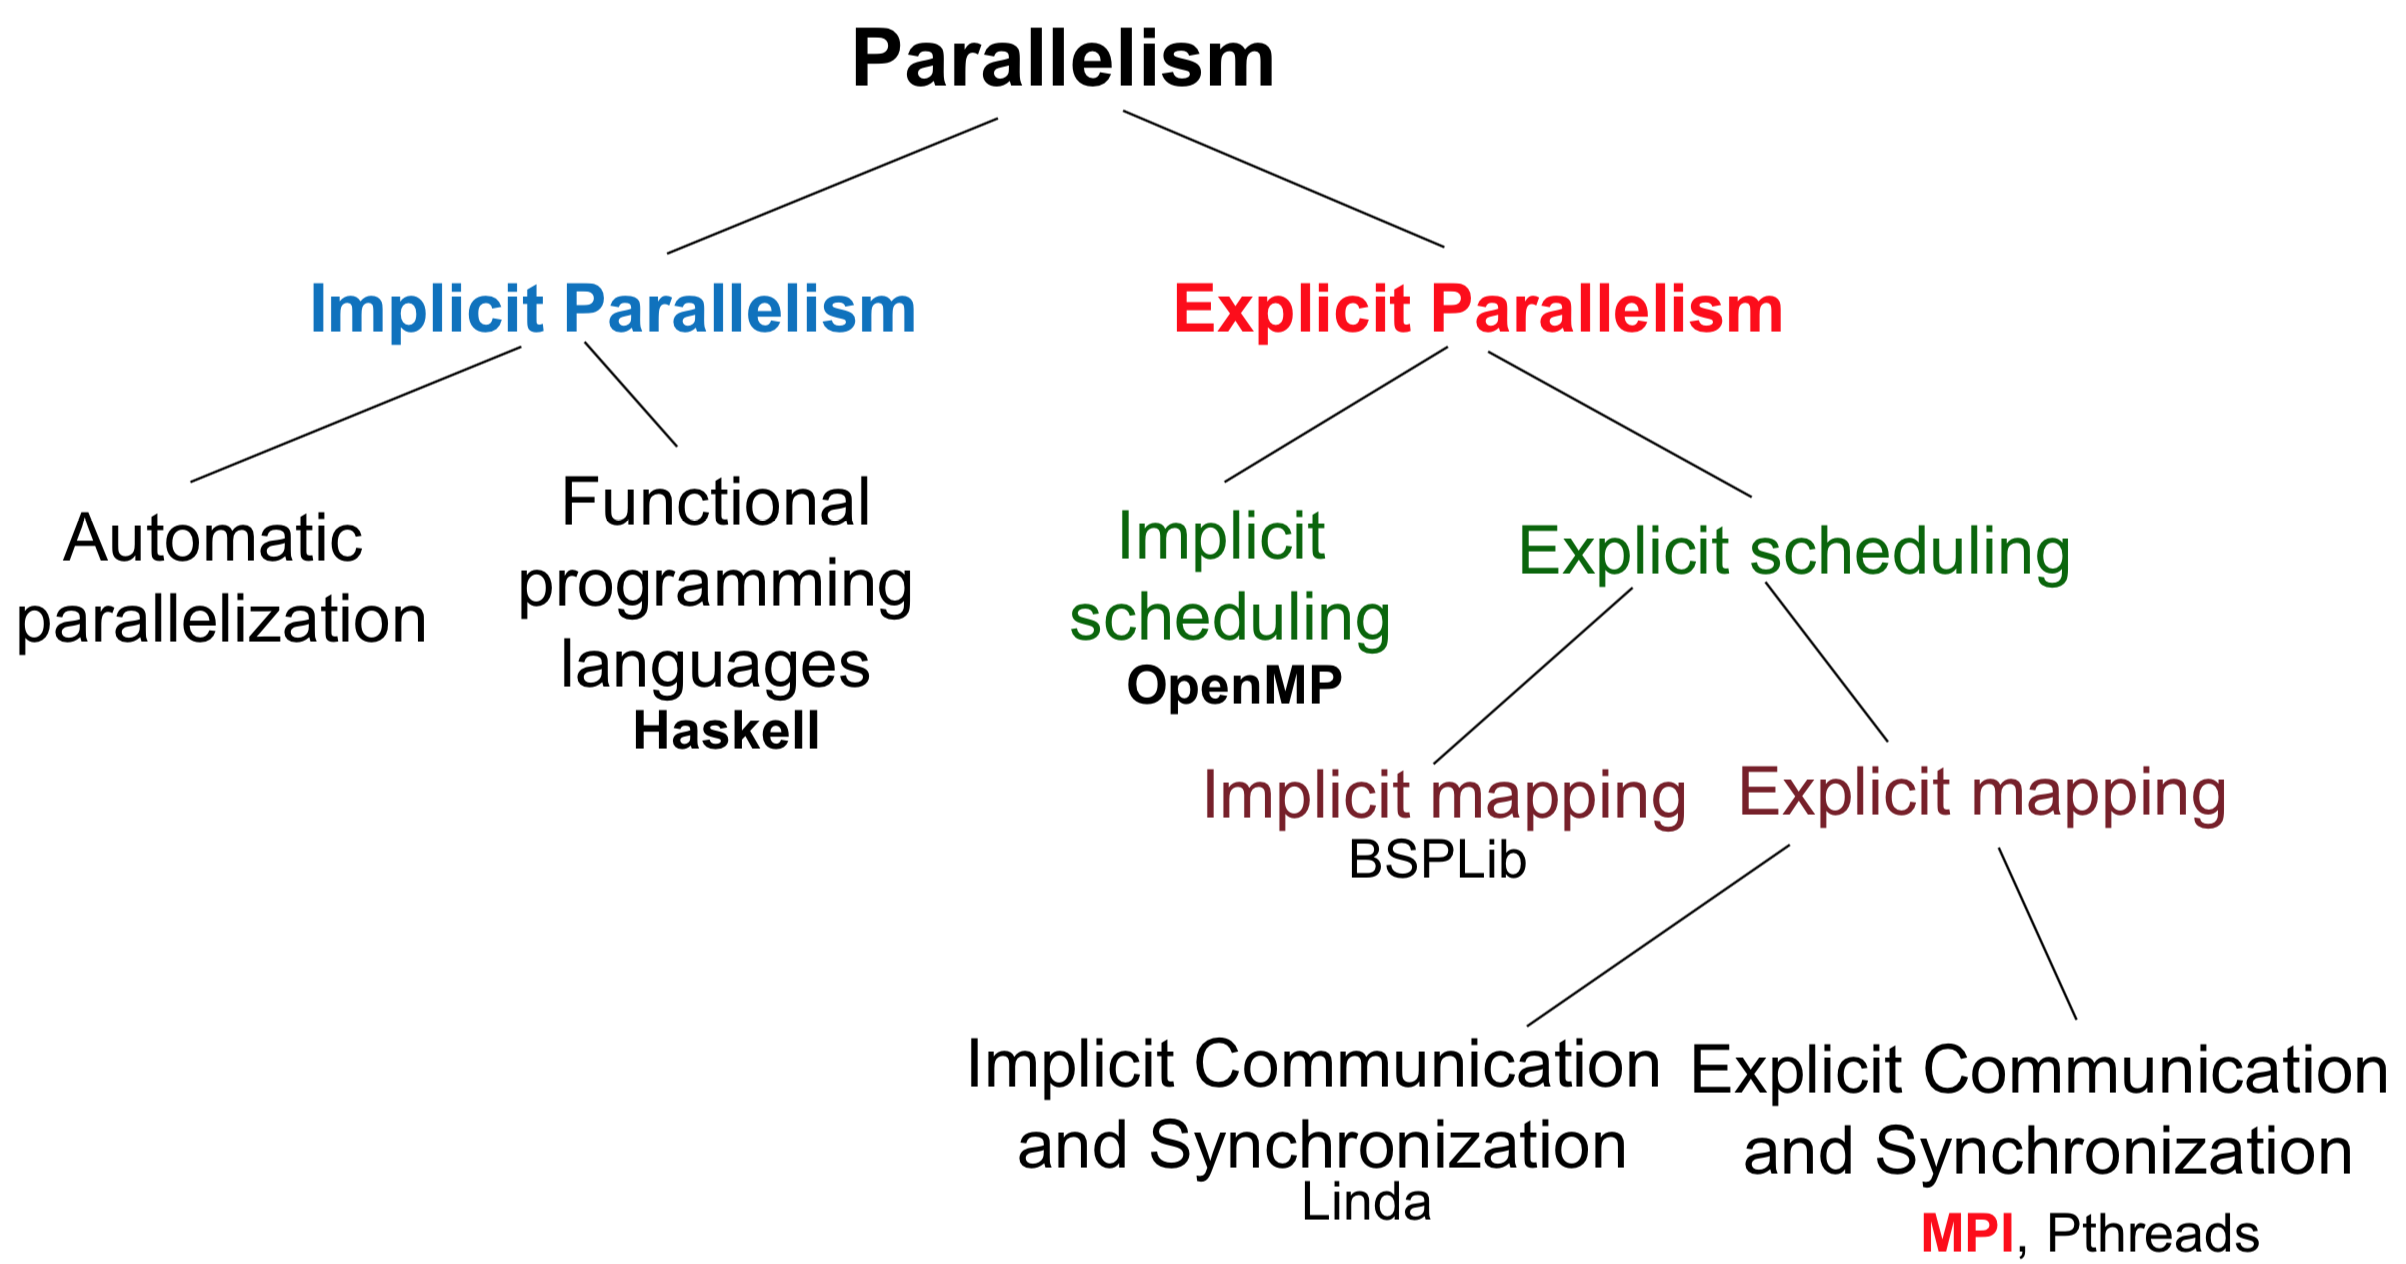
\includegraphics[width=\linewidth]{parallelism-rep}
  \end{tabularx}
  \begin{tabularx}{0.5\columnwidth}{X}
    \subsubsection{Automatic Parallelisation}
    \begin{itemize}
      \item Parallelising compilers perform decomposition \& scheduling
      \item Drawbacks: Dep analysis is diff for pointer-based computations/indirect addressing; Exec time of function calls/loops with unknown bounds is difficult to predict at compile time
    \end{itemize}
  \end{tabularx}
  \subsubsection{FP languages}
  \begin{itemize}
    \item Describe computation as eval of maths functions w/o side effects.
    \item \textbf{Advantage}: new lang constructs are not necessary to enable parallel exec
    \item \textbf{Challenge}: extract parallelism at right level of recursion
  \end{itemize}
  \subsection{Parallel Programming Patterns}
  \subsubsection{Fork-Join}Task T creates a number of child tasks with \texttt{fork()}, then waits for termination using \texttt{join} call
  \subsubsection{Parbegin-Parend}
  When an executing thread reaches parbegin-parend, a set of threads is created and statements of the construct are assigned to these threads for execution. Statements following the construct are only executed after all these threads have finished their work.
  \subsubsection{SIMD}
  Single instructions are executed synchronously by the different threads on different data
  \subsubsection{SPMD}
  Same program executed on different processors but operate on different data, No implicit synchronisation -- must use explicit sync ops
  \subsubsection{Master-Slave (or Master-Worker)}
  Master coord, init, timings, output, assigns work to slaves
  \subsubsection{Client-Server}
  \begin{itemize}
    \item MPMD (multiple program multiple data) model, useful in heterogeneous systems
    \item Server compute requests from multiple client tasks concurrently, can use multiple threads to compute a single request
    \item A task can gen requests to other tasks (client) and process requests from other tasks (server)
  \end{itemize}
  \subsubsection{Pipelining}
  Data in the application is partitioned into a stream of data elements that flows through the each of the pipeline tasks one after the other to perform different processing steps.
  \subsubsection{Task (Work) Pools}
  \begin{itemize}
    \item Common data structure from which threads can access to retrieve tasks for execution. During processing of a task, a thread can generate new tasks and insert them into the task pool.
    \item No of threads is fixed, threads created statically by main thread
    \item Access to the task pool must be synced to avoid race conditions
    \item Exec is completed when Task pool is empty, Each thread has terminated the processing of its last task
    \item \textbf{Advantages}: Useful for adaptive \& irregular applications (tasks can be generated dynamically), Overhead for thread creation is independent of problem size \& no of tasks
    \item \textbf{Disadvantages}: For fine-grained tasks, the overhead of retrieval \& insertion of tasks becomes important
  \end{itemize}
  \subsubsection{Producer-Consumer}
  \begin{itemize}
    \item Prod threads produce data which are used as input by con threads
    \item Sync must be used to ensure correct coordination b/w prod \& con
  \end{itemize}
  \section{Performance of Parallel Systems}
  \subsection{Performance factors}
  Down the list, Higher level of abstraction, higher loss in performance
  \begin{itemize}
    \item \textbf{Machine Model}: provide a description of hardware \& OS
    \item \textbf{Architectural Model}: includes interconnection network, memory org, sync/async processing, exec mode
    \item \textbf{Computational Model}: provide an analytical method for designing and evaluating algo on a given arch model
    \item \textbf{Programming Model}: define how programmer can code an algo
  \end{itemize}
  \subsubsection{Response Time in Sequential Systems}
  \begin{itemize}
    \item Wall-clock time (actual time taken) = user CPU + system CPU (OS routines) + waiting time (I/O, time sharing)
    \item Focus on CPU Time: depends on translation by compiler, exec time of each instruction
    \item $Time_{user}(A) = N_{cycle}(A) \times Time_{cycle}$, $N_{cycle}(A) = \sum\limits_{i = 1}^{n} n_i(A)\times CPI_i$
    \item Thus, $Time_{user}(A) = N_{instr}(A)\times CPI(A) \times Time_{cycle}$
    \item Refinement with memory access time:\\
          $Time_{user}(A) = (N_{cycle}(A) + N_{mm\_cycle}(A)) \times Time_{cycle}$
    \item One-level cache: $N_{mm\_cycle}(A) = N_{read\_cycle}(A) + N_{write\_cycle}(A)$, $N_{read\_cycle}(A) = N_{read\_op}(A)\times R_{read\_miss}(A) \times N_{miss\_cycles}(A)$
    \item $Time_{user}(A) = (N_{instr}(A)\times CPI(A)) + N_{rw\_op}(A)\times R_{miss}(A) \times N_{miss\_cycles} \times Time_{cycle}$ ($R_{miss}(A)$ r/w miss rate)
    \item \textbf{Average memory access time}:\\
          $T_{read\_access}(A) = T_{read\_hit} + R_{read\_miss}(A) \times T_{read\_miss}$
    \item \textbf{Two-level cache}:\\
          $T_{read\_access}(A) = T^{L1}_{read\_hit} + R^{L1}_{read\_miss}(A) \times T^{L1}_{read\_miss}$\\
          $T^{L1}_{read\_miss}(A)= T^{L2}_{read\_hit}(A) + R^{L2}_{read\_miss}(A) \times T^{L2}_{read\_miss}$\\
          Global miss rate = $R^{L1}_{read\_miss}(A) \times R^{L2}_{read\_miss}(A)$
  \end{itemize}
  \subsubsection{Throughput: MIPS (Million-Instruction-Per-Second)}
  $MIPS(A) = \frac{N_{instr}(A)}{Time_{user}(A)\times 10^6} = \frac{clock freq}{CPI(A) \times 10^6}$

  \textbf{Drawbacks}: Consider only the no of instr, easily manipulated
  \subsubsection{Million-FLoating-point-Operations-Per-Second}
  $MFLOPS(A) = \frac{N_{flops}(A)}{Time_{user}(A) \times 10^6}$, \textbf{Drawbacks}: No differentiation between diff types of flops
  \subsubsection{Benchmarks}
  \textbf{Industry Standards}: SPEC benchmark suites, EEMBC benchmark suites, Numerical Aerodynamic Simulation (NAS) from NASA (massively parallel benchmark for computer cluster), \textbf{Simple Benchmark}: Linpack, Dhrystone/Whetstone, Tak function
  \subsection{Parallel Execution Time}
  \begin{itemize}
    \item $T_p(n)$, problem of size $n$, $p$ processors
    \item Consists of Time for executing local computations, exchange of data and sync b/w processors, waiting time (unequal load distribution, wait to access shared data structure)
  \end{itemize}
  \subsubsection{Cost}
  \begin{itemize}
    \item $C_p(n) = p \times T_p(n)$ = total amount of work by all processors (processor-runtime product)
    \item \textbf{Cost optimal} = execs same total no of ops as fastest seq program
  \end{itemize}
  \subsubsection{Speedup}
  \begin{itemize}
    \item $S_p(n) = \frac{T_{best\_seq}(n)}{T_p(n)}$
    \item Theoretically, $S_p(n) \leq p$ always holds, but in practice $S_p(n)>p$ (superlinear speedup) can occur (due to better cache locality, etc.)
  \end{itemize}
  \subsubsection{Best Sequential Algo: Difficulties}
  \begin{itemize}
    \item Best sequential algo may not be known OR there exists an algo with optimum asymptotic exec time, but other algo lead to lower exec time in practice
  \end{itemize}
  \subsection{Parallel Program Efficiency}
  $E_p(n) = \frac{T_{best\_seq}}{C_p(n)} = \frac{S_p(n)}{p} = \frac{T_{best\_seq}}{p\times T_p(n)}$, Ideal $S_p(n) = p \rightarrow E_p(n) = 1$
  \subsection{Scalability}
  \subsubsection{Grosch's Law (1953)}
  The speed of a computer is proportional to the square of its cost
  \begin{itemize}
    \item Collection of smaller processors will always have less perf than a single processor of same total cost
    \item \textbf{Rebuttal}: No longer applies to computer systems build with many inexpensive commodity processors which are more cost effective than custom design supercomputers
  \end{itemize}
  \subsubsection{Minsky's Conjecture (1971)}
  Speedup achievable by parallel computer increases as log(no of processing elements)
  \begin{itemize}
    \item \textbf{Implication}: large-scale parallelism unproductive
    \item \textbf{Rebuttal}: Experimental results prove that speedup depends strongly on particular algo \& computer arch, and many algo exhibit linear speedup for over 100 processors
  \end{itemize}
  \subsubsection{Amdahl's Law (1967)}
  Speedup of parallel execution is limited by the fraction of the algo that can't be parallelised
  \begin{itemize}
    \item $0 \leq f \leq 1$ = sequential fraction (fixed-workload performance)
    \item $S_p(n) = \frac{T_{best\_seq}(n)}{f\times T_{best\_seq}(n)+\frac{1-f}{p}T_{best\_seq}(n)}$
    \item Implication: manufacturers are discouraged from making large parallel computers, more research attn shifted towards developing parallelising compilers that reduces $f$
    \item \textbf{Rebuttal}: in many computing problems, $f$ is not constant, dependent on problem size $n$. An effective parallel algorithm is $\lim\limits_{n\rightarrow\infty}f(n) = 0$, thus speedup $\lim\limits_{n\rightarrow\infty}S_p(n)=\frac{p}{1+(p-1)f(n)}=p$, thus Amdahl's law can be circumvented for large problem size
  \end{itemize}
  \subsubsection{Gustafson's Law (1988)}
  \begin{itemize}
    \item Main constraint is exec time, then higher computing power is used to improve accuracy/better result
    \item If $f$ decreases when $n$ increases, then $S_p(n) \leq p$, $\lim\limits_{n\rightarrow\infty}S_p(n)=p$
  \end{itemize}
  \section{Coherence, Consistency, Interconnections}
  \subsection{Cache}
  \subsubsection{Write Policy}
  \begin{itemize}
    \item \textbf{Write-through} - write immediately transferred to main memory, Advantage: no stale value, disadv: slow (soln: use a write buffer)
    \item \textbf{Write-back} - write op performed only in the cache, write performed only when cache block is replaced, tracked with a dirty bit. Adv: less write ops, disadv: mem may contain invalid entries
  \end{itemize}
  \subsubsection{Cache Coherence Problem}
  3 properties of coherent memory system:
  \begin{enumerate}
    \item $P$ write to $X$, no write to $X$, $P$ read from $X$, should be same value
    \item $P_1$ write to $X$, no write ro $X$, $P_2$ read from $X$, should be same value (\textbf{Write Propagation})
    \item Write $v_1$ to $X$, write $v_2$ to $X$, processors read same order ($v_1$ then $v_2$) (\textbf{Write Serialisation})
  \end{enumerate}
  \subsubsection{Maintaining cache coherence}
  \begin{itemize}
    \item Software-based soln (compiler+hw aided soln)
    \item Hardware-based soln (most common on multiprocessor, \textbf{cache coherence protocols})
  \end{itemize}
  Major Tasks:
  \begin{itemize}
    \item \textbf{Track cache line sharing status}, 2 major categories:
          \begin{itemize}
            \item \textbf{Snooping-based}: no centralised directory, each cache keeps track of the sharing status, cache \textbf{monitors/snoops} on the bus to update the status of cache line \& take appropriate action. Most common in arch with a bus. Granularity is cache block.
                  \begin{itemize}
                    \item All the processors on the bus can observe every bus transactions (\textbf{write propagation}), Bus transactions visible to the processors in the same order (\textbf{write serialisation})
                  \end{itemize}
            \item \textbf{Directory based}: sharing status kept in a centralised location. Most common in NUMA
          \end{itemize}
    \item Handle the update to a shared cache line (maintain coherence)
  \end{itemize}
  \subsection{Memory Consistency Models}
  4 types of memory op orderings: RAW, RAR, WAR, WAW
  \subsubsection{Sequential Consistency}
  Maintains all four orderings
  \begin{itemize}
    \item Every processor issues its mem ops in program order
    \item Mem accesses are atomic (effect of each mem op must be visible to all before next mem op)
  \end{itemize}
  \subsubsection{Total Store Ordering (TSO)}
  \begin{itemize}
    \item Relaxing RAW (WAW still exists, writes by same thread in-order)
    \item Processor $P$ can read $B$ before its write to $A$ is seen by all (processor can move its own reads in front of its own writes)
    \item Read by other processors cannot return new value of $A$ until write to $A$ is observed by all processors
  \end{itemize}
  \subsubsection{Processor Consistency}
  \begin{itemize}
    \item Relaxing RAW (WAW still exists, writes by same thread in-order)
    \item Any processor can read new value of $A$ before the write is observed by all processors
  \end{itemize}
  \subsubsection{Partial Store Ordering}
  \begin{itemize}
    \item Relaxing RAW \& WAW, but still guarantees write atomicity
  \end{itemize}
  \subsection{Interconnection Networks}
  \subsubsection{Shearsort}
  \begin{enumerate}
    \item Row sorting, odd rows sort asc, even rows sort desc
    \item Column sorting, all columns sort asc
    \item Repeat until sorted
  \end{enumerate}
  For $n$ numbers, $log(n)$ phases, $O(\sqrt{n}\log n)$. Good for 2D mesh network, only comm w/ adj nodes.
  \subsection{Topology}
  \subsubsection{Metric}
  \begin{itemize}
    \item \textbf{Diameter}: max dist b/w any pair of nodes (small diameter, small dist for msg transmission)
    \item \textbf{Degree}: no of direct neighbour nodes (small node degree reduces node h/w overhead)
    \item \textbf{Bisection width}: min. no. of edges to be removed to divide the network into 2 equal halves. (measure for capacity of network when transmitting messages simulatenously)
    \item \textbf{Node connectivity}: min. no of nodes failing to disconnect network (network robustness)
    \item \textbf{Edge connectivity}: min. no of edges failing to disconnect network (no of independent paths b/w any pair of nodes)
  \end{itemize}
  \subsubsection{Direct Interconnection (Static/Point-To-Point)}
  Torus = 2 links for every dim, Mesh = torus w/ no wraparound, CCC = k-dim hypercube but each node replaced with cycle of k-nodes\\
  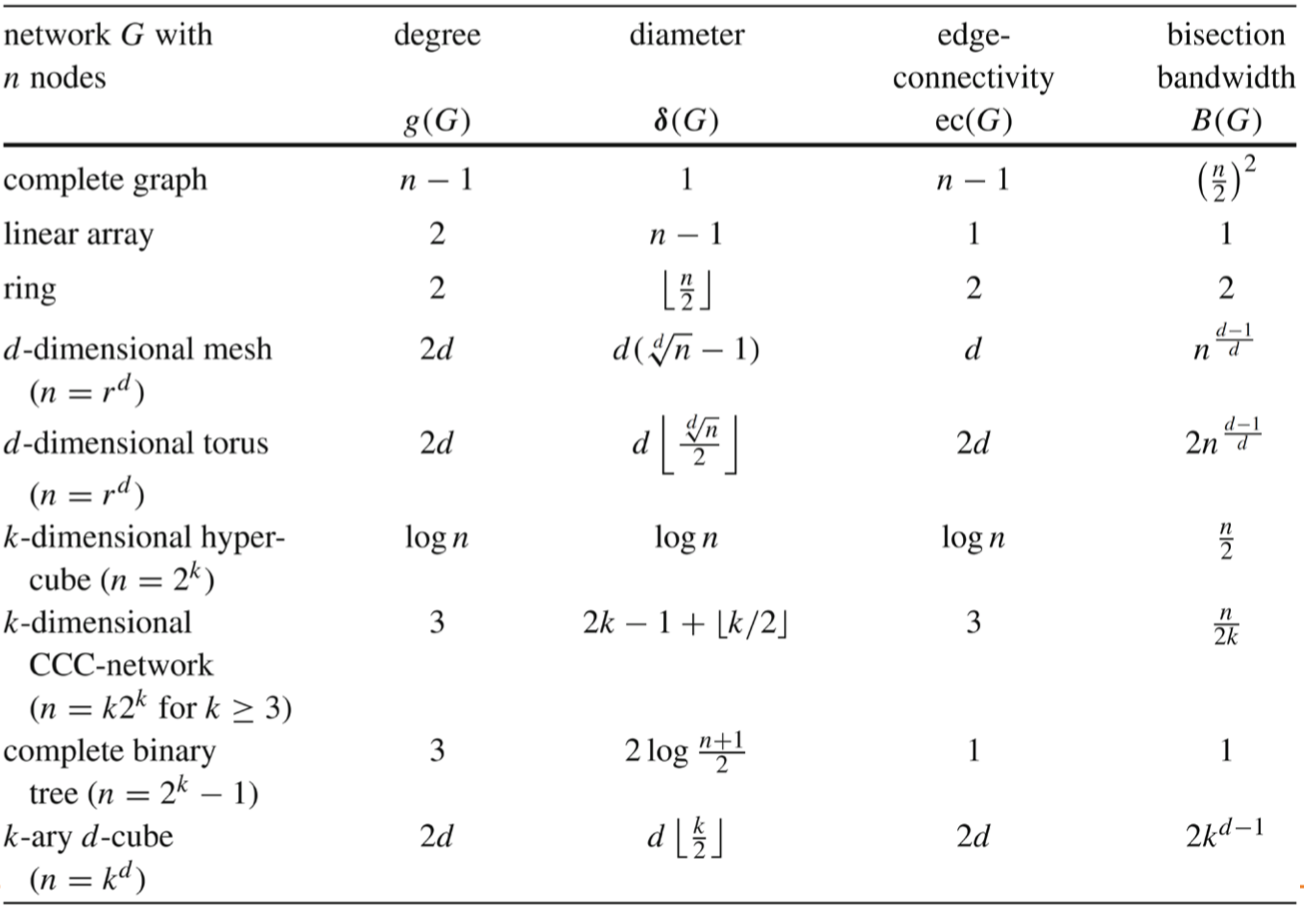
\includegraphics[width=\linewidth]{topology}
  \subsubsection{Indirect Interconnection (using switches) - examples for 8 to 8}
  \begin{itemize}
    \item \textbf{Bus Network} -- a set of wires, only one pair of devices can communicate at a time, bus arbiter for coordination
    \item \textbf{Crossbar Network} has $n\times m$ switches for $n$ in, $m$ out. Switch = either straight/change dir
    \item \textbf{Omega Network} -- 1 unique path for every input to output, Uses $\log n$ stages, $\frac{n}{2}$ switches/stage. Edge from node $(\alpha, i)$ to two nodes $(\beta, i + 1)$ where $\beta = \alpha$ by a cyclic left shit (+ inversion of the LSBit)
    \item \textbf{Butterfly Network} -- Node $(\alpha, i)$ connects to $(\alpha, i + 1)$ and $(\alpha', i + 1)$, $\alpha$ and $\alpha'$ differ in the (i+1)th bit from the left (cross edge)
    \item \textbf{Baseline Network} -- Node $(\alpha, i)$ connects to 2 nodes $(\beta, i + 1)$ where $\beta = $ cyclic right shift of last (k-1) bits of $\alpha$ OR inversion of the LSBit of $\alpha$ + cyclic right shift of last (k-i) bits.
  \end{itemize}
  \begin{tabularx}{0.35\linewidth}{X}
    Omega \\
    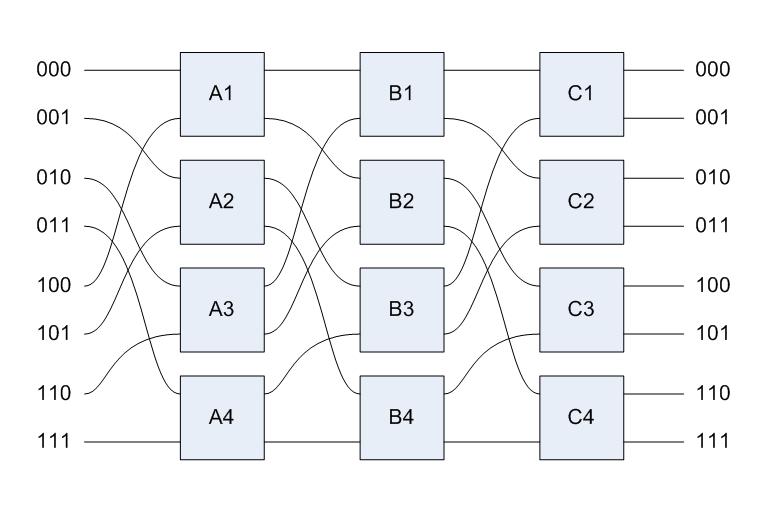
\includegraphics[width=\linewidth]{omega}
  \end{tabularx}
  \begin{tabularx}{0.3\linewidth}{X}
    Butterfly \\
    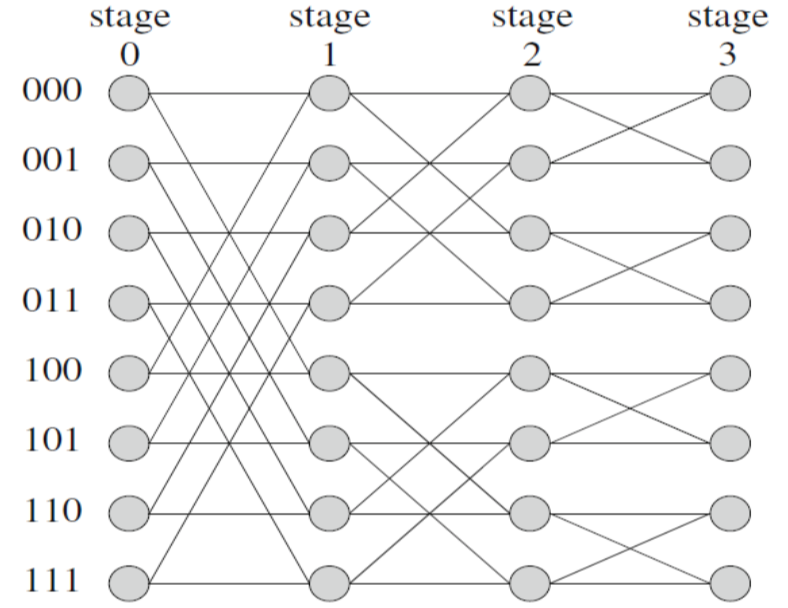
\includegraphics[width=\linewidth]{butterfly}
  \end{tabularx}
  \begin{tabularx}{0.3\linewidth}{X}
    Baseline \\
    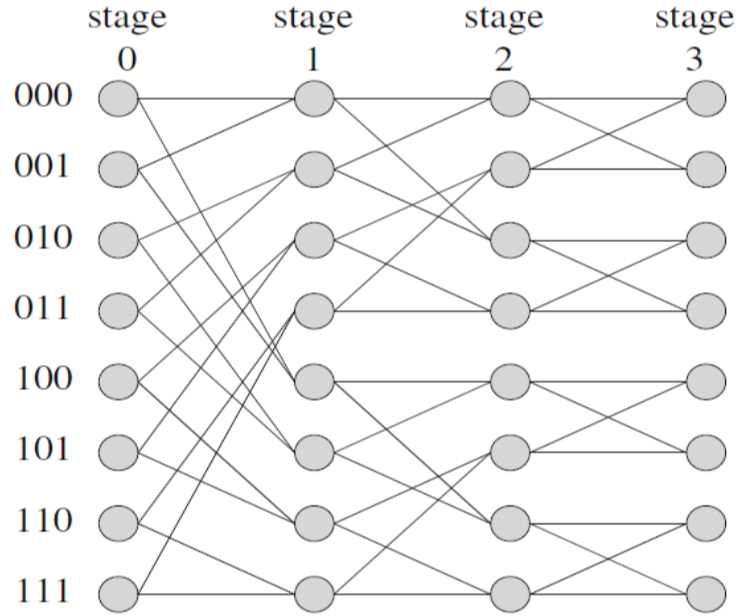
\includegraphics[width=\linewidth]{baseline}
  \end{tabularx}
  \subsection{Routing}
  Based on:
  \begin{itemize}
    \item Path length (minimal/non-minimal) whether shortest path
    \item Adaptivity (deterministic/adaptive) whether always the same path for same pair of nodes/take into account network status
  \end{itemize}
  \subsubsection{XY Routing for 2D Mesh (Deterministic)}
  $(X_{src}, Y_{src})$ to $(X_{dst}, Y_{dst})$: move in x-direction until $X_{src} = X_{dst}$, then move in y-direction
  \subsubsection{E-Cube Routing for Hypercube (Deterministic)}
  No of bits difference b/w 2 pairs of nodes = number of hops (hamming distance). Start from MSB to LSB (vice versa), find first different bit, go to neighbouring node with the bit corrected.
  \subsubsection{XOR-Tag Routing for Omega Network (Deterministic)}
  $T =$ Source Id $\oplus$ (XOR) Destination ID

  A t stage-$k$: go straight if bit $k$ of $T$ is $0$, crossover if bit $k$ of $T$ is $1$

  \section{Parallel Programming Models}
  \subsection{Data Distribution}
  \textbf{Assumptions:} $p$ identical processors, array starts from 1, Block size = B = $\left\lceil\frac{n}{p}\right\rceil$
  \subsubsection{1D Array}
  \begin{itemize}
    \item \textbf{Blockwise}: $P_i$ takes elements [$(j-1)\times B + 1$, ..., $j\times B$]
    \item \textbf{Cyclic}: $P_i$ takes elements [$j$, $j + p$, ..., $j+(B-1)\times p$] if $j \leq n \mod p$, else [$j$, $j + p$, ..., $j + (B - 2)\times p$]
  \end{itemize}
  \subsubsection{2D Array}
  \begin{itemize}
    \item Combination of blockwise/cyclic in 1/both dimension(s)
    \item 1D distribution: column-wise blockwise, cyclic, or block-cyclic (Form blocks of size $b$, then perform round-robin cyclic allocation)
  \end{itemize}
  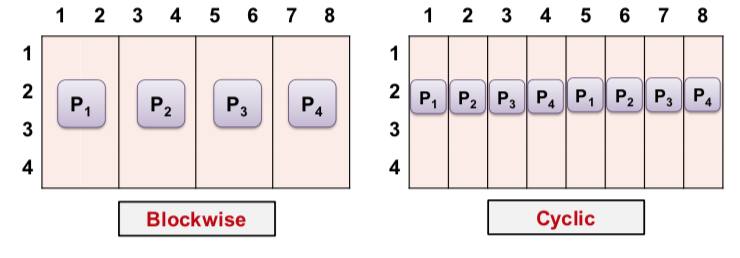
\includegraphics[width=0.55\linewidth]{2d-1}
  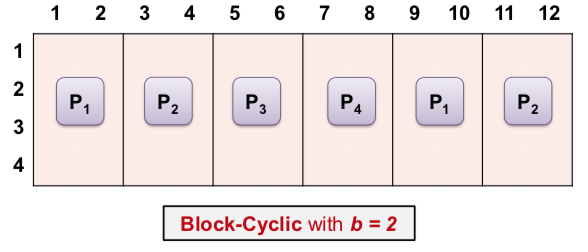
\includegraphics[width=0.45\linewidth]{2d-2}
  \begin{itemize}
    \item Checkerboard distribution
  \end{itemize}
  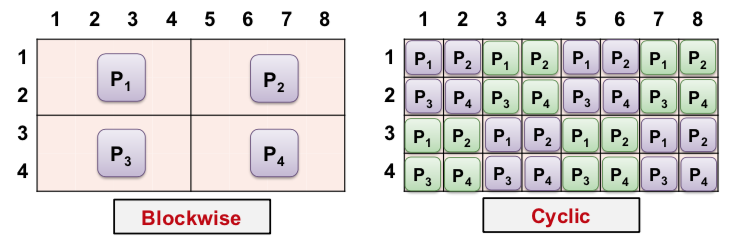
\includegraphics[width=0.55\linewidth]{2d-3}
  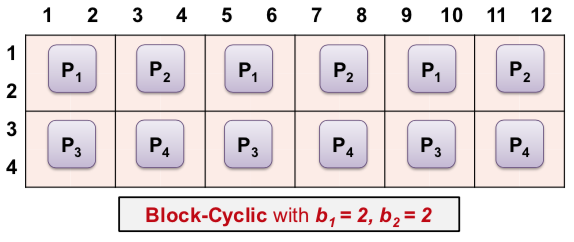
\includegraphics[width=0.45\linewidth]{2d-4}
  \subsection{Information Exchange}
  For controlling coordination of different parts of a parallel program execution
  \subsubsection{Shared Address Space (Shared variables)}
  Assumes a global memory accessible by all processors, need sync ops for safe concurrent access to prevent race condition using mutex to protect critical section, e.g. \mintinline{C}{#pragma omp critical {}} or \mintinline{C}{omp_init_lock(omp_lock_t*)}, \mintinline{C}{omp_set_lock}, \mintinline{C}{omp_unset_lock}
  \subsubsection{Distributed Address Space (Communication operations)}
  \begin{itemize}
    \item Assumes disjoint memory space -- data exchange through dedicated comm ops
    \item 2 main types of data exchange: point-to-point and global communication
    \item Examples:
          \begin{itemize}
            \item \textbf{Single transfer}: point-to-point, \texttt{send} and \texttt{receive}
            \item \textbf{Scatter/Gather}: takes elements and distributes them in order of process rank
            \item \textbf{Single Broadcast}: takes a single data element at the root and copies it to all other
            \item \textbf{Multi Broadcast}: (\texttt{MPI\_Allgather}) "Gather + Single Broadcast"
            \item \textbf{Single accumulation}: reduction (binary, associative, commutative) op applied to all elements, result stored in root (Gather + Reduce)
            \item \textbf{Multi accumulation}: "Accumulation + Scatter"
            \item \textbf{Total Exchange}: (\texttt{MPI\_Alltoall}) "transpose"
          \end{itemize}
  \end{itemize}
  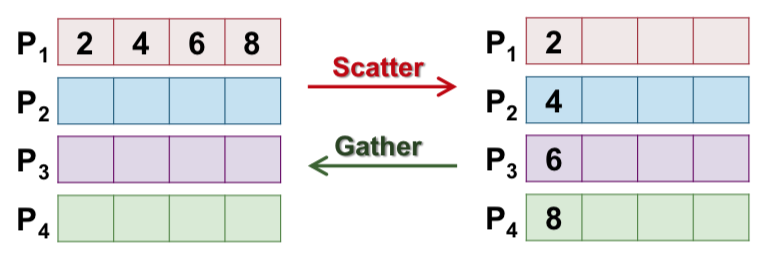
\includegraphics[width=0.33\linewidth]{scattergather}
  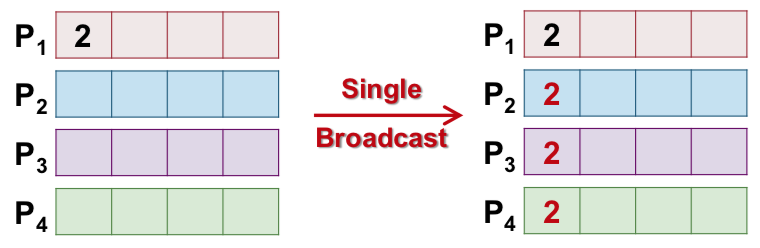
\includegraphics[width=0.33\linewidth]{singlebcast}
  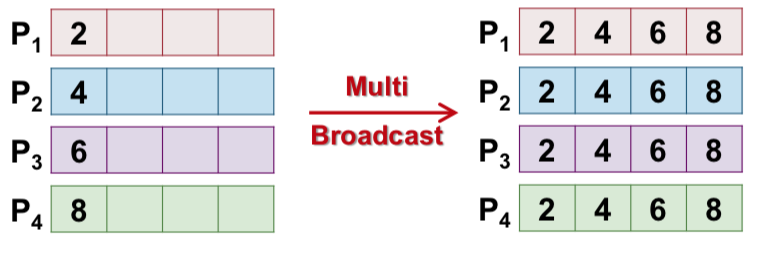
\includegraphics[width=0.33\linewidth]{multibcast}
  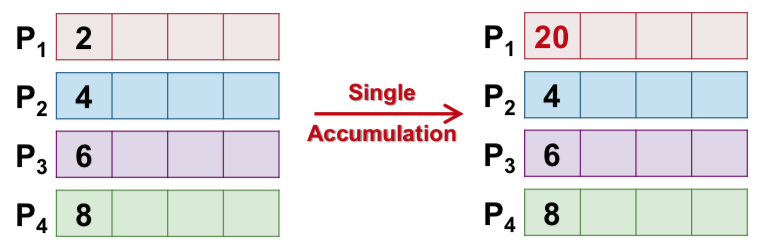
\includegraphics[width=0.33\linewidth]{singleaccu}
  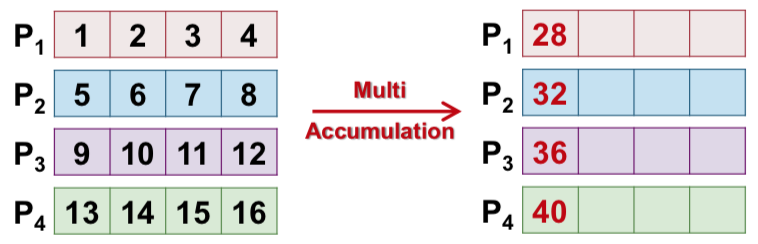
\includegraphics[width=0.33\linewidth]{multiaccu}
  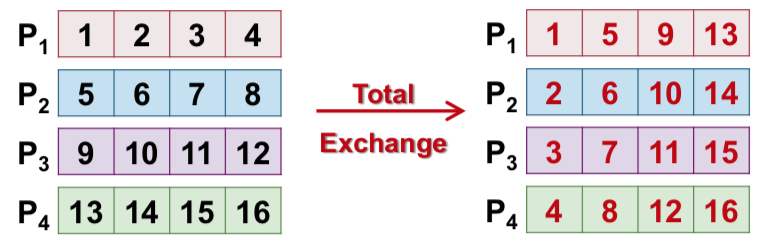
\includegraphics[width=0.33\linewidth]{totalexch}
  \begin{itemize}
    \item \textbf{Duality of comm ops}: interconnection can be represented by a spanning tree. Duality if the same spanning tree can be used for both ops
  \end{itemize}
  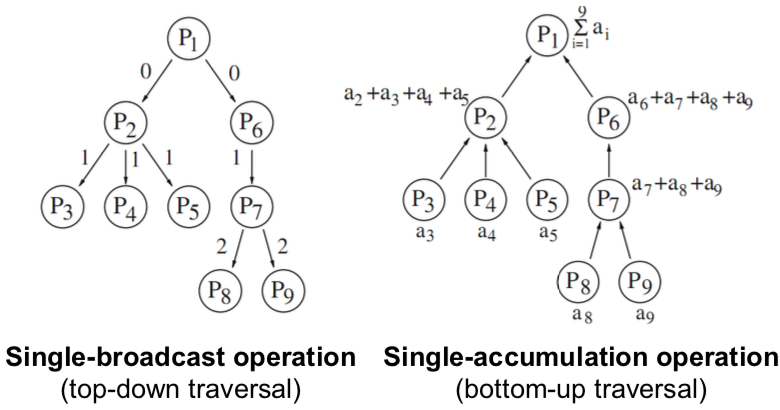
\includegraphics[width=0.5\linewidth]{duality1}
  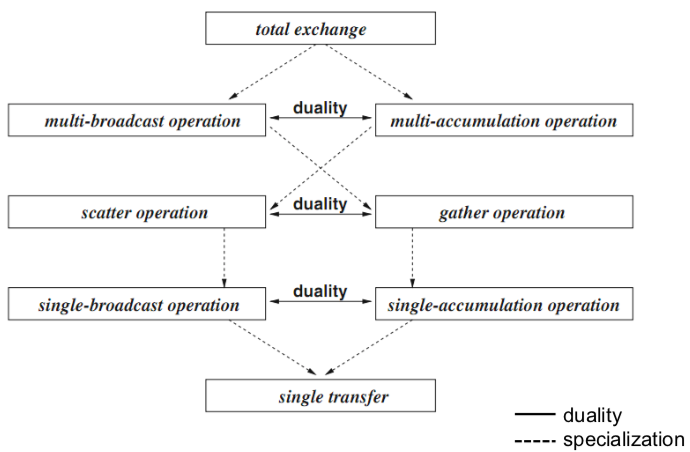
\includegraphics[width=0.5\linewidth]{duality2}
  \section{Message Passing Programming}
  Loosely synchronous paradigm, tasks sync to perform interactions, but otherwise exec is async: \textbf{SPMD} (Single Program Multiple Data) model
  \begin{tabularx}{\columnwidth}{l | X | X}
                           & \textbf{Blocking}                                                            & \textbf{Non-Blocking}                                                                \\ \hline
    \textbf{Buffered}      & Sending process returns after data has been copied into comm buffer          & Sending process returns after initiating DMA transfer to buffer, may not be complete \\ \hline
    \textbf{Non-bufferred} & Sending process blocks until matching receive operation has been encountered &                                                                                      \\
  \end{tabularx}
  \begin{itemize}
    \item \textbf{Blocking} = send op blocks until it is safe. Issue: deadlock
    \item \textbf{Non-blocking} = send/recv returns before it is safe -- generally accompanied by a check-status op. Used correctly, can overlap comm overheads with useful computations
    \item \textbf{Non-buffered}, issues: idling (timing mismatch sender <-> recvr)
    \item \textbf{Buffered}: buffers at both ends, trades idling overhead for buffer copying overhead
  \end{itemize}
  Summary = \textbf{Overhead}: idling (non-buffered) vs buffer management (buffered), \textbf{Side effect}: safe and easier programming (blocking) vs hiding comm overhead (non-blocking)
  \subsection{Message Passing Interface (MPI)}
  \subsubsection{Semantic, Local View}
  \begin{itemize}
    \item \textbf{Blocking}: return from lib call indicates user is allowed to reuse resources specified
    \item \textbf{Non-blocking}: may return before op completes, before user is allowed to reuse resources
  \end{itemize}
  \subsubsection{Semantic, Global View}
  \begin{itemize}
    \item \textbf{Synchronous}: comm op doesn't complete before both processes have started their comm op
    \item \textbf{Asynchronous}: sender can execute its comm op without any coordination with the receiver
  \end{itemize}
  \begin{tabularx}{\columnwidth}{l | X | X}
                          & \textbf{Synchronous}                       & \textbf{Asynchronous}                    \\ \hline
    \textbf{Blocking}     & \texttt{MPI\_SSend}, \texttt{MPI\_SRecv}   & \texttt{MPI\_Send}, \texttt{MPI\_Recv}   \\ \hline
    \textbf{Non-blocking} & \texttt{MPI\_ISSend}, \texttt{MPI\_ISRecv} & \texttt{MPI\_ISend}, \texttt{MPI\_IRecv}
  \end{tabularx}
  \subsubsection{Initialisation, Finalisation, Abort}
  \begin{itemize}
    \item \mintinline{C}{int MPI_Init(int* argc, char** argv[])}, initialise MPI program, called only once
    \item \mintinline{C}{int MPI_Finalize(void)}, terminate all MPI processing, last MPI call
    \item \mintinline{C}{int MPI_Abort(MPI_Comm comm, int errorCode)}, force all processes to terminate, return errorCode to \texttt{mpirun}
    \item Other functions: \texttt{MPI\_Comm\_size}, \texttt{MPI\_Comm\_rank}
  \end{itemize}
  \subsubsection{MPI Messages Format}
  \begin{itemize}
    \item \textbf{Message} = data + envelope (how to route the data)
    \item \textbf{Data} = start-buffer (pointer to data) + count + datatype
    \item \textbf{Envelope} = destination/source (using rank in a communicator) + tag (arbitrary number to distinguish messages) + communicator
  \end{itemize}
  \subsubsection{Process Group}
  \begin{itemize}
    \item An ordered set or processes where each process has a unique rank
    \item A process may be member of multiple groups (and may have diff ranks in each of these groups) -- handled by MPI
  \end{itemize}
  \subsubsection{Communicator}
  \begin{itemize}
    \item Communication domain for a group of processes
    \item 2 types: \textbf{Intra-communicators} (supports the execution of arbitrary collective comm op on a single group, default: \texttt{MPI\_COMM\_WORLD}), \textbf{Inter-communicators} (supports the point-to-point comm op b/w 2 process groups)
    \item Allows to organise tasks based on func into task groups, Enable collective communication operations across a subset of related tasks, Provide basis for user-defined virtual topologies
  \end{itemize}
  \subsubsection{Process Virtual Topologies}
  \begin{itemize}
    \item A communicator with a Cartesian style of addressing the ranks of the processes
    \item \texttt{MPI\_Cartdim\_get} and \texttt{MPI\_Cart} prefix: \texttt{create}, \texttt{get}, \texttt{coords}, \texttt{rank}, \texttt{shift}
  \end{itemize}
  \subsubsection{MPI Point-to-Point communication}
  \begin{tabularx}{0.6\linewidth}{X}
    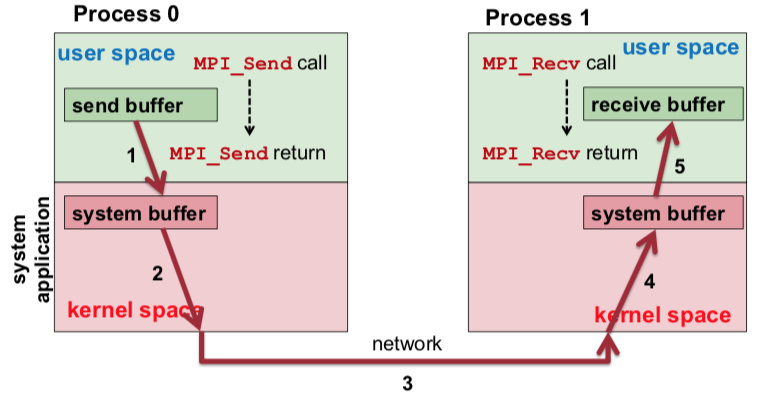
\includegraphics[width=\linewidth]{mpi}
  \end{tabularx}
  \begin{tabularx}{0.4\linewidth}{X}
    Messages to one particular destination are delivered in the order they are sent. \\
    \\
    No guarantee for multiple messages to multiple destinations
  \end{tabularx}
  \subsubsection{Deadlocks}
  \begin{verbatim}
MPI_Recv(recvbuf, ...);          MPI_Recv(recvbuf, ...);
MPI_Send(sendbuf, ...);          MPI_Send(sendbuf, ...);
\end{verbatim}
  \begin{itemize}
    \item For \texttt{MPI\_Recv}, as above
    \item For \texttt{MPI\_Send}, occurs when runtime doesn't use system buffers/system buffers are too small.
    \item \textbf{Deadlock-free logical ring}: procs w/ even rank: send -> receive; odd rank: receive -> send
  \end{itemize}
  \subsubsection{Collective Communication}
  \begin{tabularx}{0.5\linewidth}{X}
    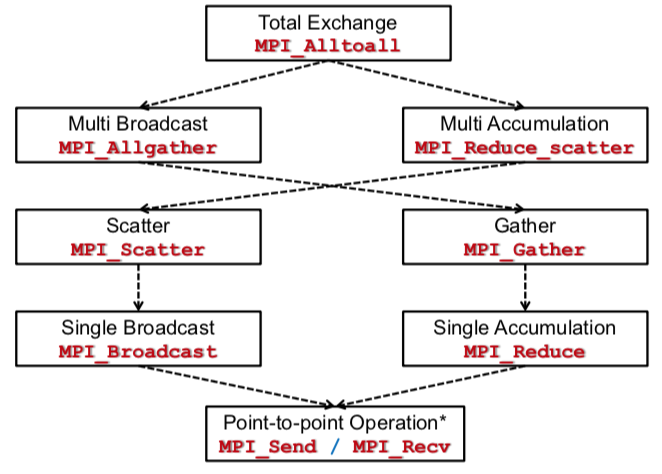
\includegraphics[width=\linewidth]{mpicollective}
  \end{tabularx}
  \begin{tabularx}{0.5\linewidth}{X}
    \begin{itemize}
      \item Operations involving all procs in a communicator, blocking by default
      \item \textbf{Scatter}: one-to-many
      \item \textbf{Gather}: many-to-one (with/without accumulation)
      \item \texttt{int MPI\_Barrier(MPI\_Comm);} the only collective sync op -- all procs must execute, blocks until all procs reach the barrier
    \end{itemize}
  \end{tabularx}
  \subsubsection{Measuring Program Timing}
  \begin{itemize}
    \item \mintinline{C}{double MPI_Wtime(void)} Time in seconds since an arbitrary time in the past.
    \item \mintinline{C}{double MPI_Wtick(void)} Time in seconds of resolution of \texttt{MPI\_Wtime}
  \end{itemize}
  \section{CUDA Programming}
  \subsection{GPU Architecture}
  \begin{itemize}
    \item Multiple \textbf{Streaming Multiprocessors} (SMs) -- memory, cache, connecting interface
    \item SM consists of multiple compute cores, memories (registers, L1 cache, texture memory, shared memory), logic for thread \& instruction management
  \end{itemize}
  \subsection{CUDA Kernel and Threads}
  \begin{itemize}
    \item \textbf{Device} = GPU, \textbf{Host} = CPU, \textbf{Kernel} = function that runs on device
    \item Parallel portions execute on device as kernels, one kernel at a time, 1 kernel = many threads
    \item CUDA threads are extremely lightweight, very little creation overhead, instant switching
    \item All threads run the same code -- SPMD (Single Program Multiple Data)
  \end{itemize}
  \subsection{Thread Cooperation}
  \begin{itemize}
    \item Share results to save computation, share memory accesses to reduce bandwidth
    \item Divide monolithic thread array into multiple blocks
    \item In a block: \textbf{shared memory, atomic ops, barrier sync}. Threads in diff blocks can't cooperate
    \item HW is free to schedule thread blocks to any processor at any time
  \end{itemize}
  \subsection{Thread Hierarchy}
  \begin{itemize}
    \item A kernel is executed by a grid of thread blocks. A block executes on 1 SM, does not migrate.
    \item Several blocks can reside concurrently on 1 SM, limited by control limitations (32 blocks/SM, 1024 threads/block) and resources (register file and shared memory are partitioned among all resident threads)
  \end{itemize}
  \subsection{Thread Execution Mapping to Architecture}
  \begin{itemize}
    \item SIMT (Single Instruction Multiple Thread) execution model
    \item SM creates, manages, schedules, executes threads in SIMT warps (group of 32 parallel threads). Threads in a warp start together at the same program address. A block is always split into warps the same way
    \item Warp executes 1 common instruction at a time. Scheduler optimises by grouping threads with the same exec paths in the same SIMT unit
  \end{itemize}
  \subsection{CUDA Memory Model}
  \begin{tabularx}{\columnwidth}{l|l|l|l|l|l}
    \textbf{Memory} & \textbf{Location} & \textbf{Cached} & \textbf{Access} & \textbf{Scope}       & \textbf{Lifetime} \\ \hline
    Register        & on chip           & n/a             & R/W             & 1 thread             & thread            \\ \hline
    Local           & off chip          & No              & R/W             & 1 thread             & thread            \\ \hline
    Shared          & on chip           & n/a             & R/W             & All threads in block & block             \\ \hline
    Global          & off chip          & No              & R/W             & All threads + host   & host alloc        \\ \hline
    Constant        & off chip          & Yes             & R               & All threads + host   & host alloc        \\ \hline
    Texture         & off chip          & Yes             & R               & All threads + host   & host alloc        \\
  \end{tabularx}
  \begin{itemize}
    \item \textbf{Shared} = higher bandwidth and lower latency than local/global. Divided into equal-sized mem mods called \textbf{banks}. Access to diff banks can be simultaneous. \textbf{Bank conflict}: mem request in the same bank, has to be serialised
    \item \textbf{Local}: automatic array vars alloc by compiler, \textbf{Texture}: for spatially coherent random-access r/o data (provides filtering, address clamping, wrapping)
  \end{itemize}
  \subsection{Programming in CUDA}
  \begin{itemize}
    \item \textbf{Func qual}: \mintinline{C}{__host__}, \mintinline{C}{__device__}, \mintinline{C}{__global__}, \textbf{Launching kernel:} \mintinline{C}{kernel<<<80, 64>>>}, \textbf{Var qual:} \mintinline{C}{__device__}, \mintinline{C}{__constant__}, \mintinline{C}{__shared__}, \textbf{unqualified}: scalar, built-in vector  stored in registers, arrays of more than 4 elements orruntime indices stored in local mem
    \item \textbf{Thread synchronisation}: \mintinline{C}{void __syncthreads()}, generates barrier sync instruction
  \end{itemize}
  \subsection{Memory Optimisations}
  Minimise data transfer between host and device mem, use page-locked/pinned mem transfer. Overlapping async transfers with GPU computations
  \subsubsection{Coalesced access to Global Mem}
  Simultaneous accesses to global mem by threads in a half-warp can be coalesced into as few as a single mem txn of 32, 64, or 128 bytes
  \subsubsection{Overall Memory Optimisations}
  Minimize data transfer between host and device, Ensure global memory accesses are coalesced whenever possible, Minimize global memory accesses by using shared memory, Minimize bank conflicts in shared memory accesses
  \subsection{Overall Optimisation}
  \begin{itemize}
    \item \textbf{Maximise parallel exec}: restructure algo to expose as much data parallelism as possible, map to HW carefully choosing exec config of each kernel invocation
    \item \textbf{Optimizing memory usage} to achieve maximum memory bandwidth: diff mem spaces and access patterns
    \item \textbf{Optimizing instruction usage} to achieve maximum instruction throughput: Use high throughput arithmetic instructions, avoid diff exec paths within the same warp
  \end{itemize}
  \section{Parallel Algorithm Design}
  \subsection{Overheads of Parallelism}
  \textbf{Tradeoff}: task granularity -- small to reduce overhead, large to still have enough parallel work
  \subsection{General Design Approach}
  \begin{itemize}
    \item Consider machine independent issues before machine specific aspects of design
    \item Task/Channel model: \textbf{Tasks} interact by sending messages through \textbf{channels}
  \end{itemize}
  \subsection{Foster's Design Methodology}
  \subsubsection{Partitioning}
  \begin{itemize}
    \item Divide \textbf{computation} \& \textbf{data} into independent pieces to discover max parallelism.
    \item Data centric -- \textbf{Domain decomposition}: divide data into pieces of approx. equal size, determine how to associate computations with the data
    \item Computation centric -- \textbf{Functional decomposition}: divide computation into pieces, determine how to associate data with the computations.
    \item \textbf{Rules of thumb}: at least 10x more primitive tasks than processors, minimise redundant computations and data storage, primitive tasks roughly same size, no of tasks an increasing function of problem size
  \end{itemize}
  \subsubsection{Communication}
  \vspace{-1mm}
  \begin{tabularx}{0.5\linewidth}{X}
    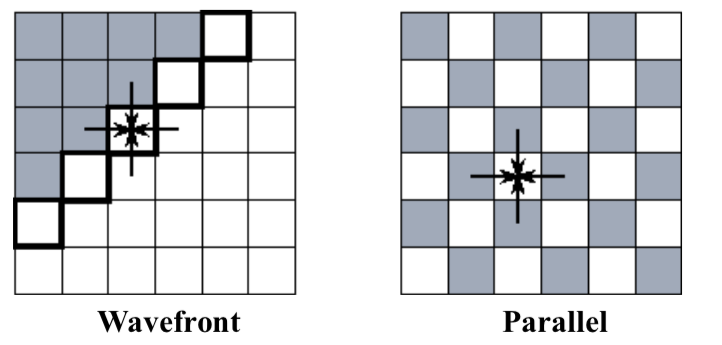
\includegraphics[width=\linewidth]{localcomm}
  \end{tabularx}
  \begin{tabularx}{0.5\linewidth}{X}
    \begin{itemize}
      \item \textbf{Local communication}: task needs data from a small no of other tasks ("neighbours"), create channels illustrating data flow
      \item \textbf{Global communication}: significant no of tasks contribute data to perform a computation, don't create channels for them early in design
      \item Ideally, distribute and overlap computation and communication
    \end{itemize}
  \end{tabularx}
  \begin{itemize}
    \item Local comm: 2 finite diff update strategies. Parallel: time t unshaded, time (t+1) shaded
    \item Global comm: optimisation through pipeline/divide-and-conquer
  \end{itemize}
  \subsubsection{Agglomeration}
  \begin{itemize}
    \item Combine tasks into larger tasks to improve perf (reduce task creation and comm overhead), maintain scalability, simplify programming
    \item In MPI, goal: create 1 agglomerated task/processor
    \item E.g. reduce dim of decomposition from 3 to 2, \textbf{3D decomposition}: combine adjacent tasks, \textbf{divide-and-conquer}: coalesce sub-trees, \textbf{tree algo} -- nodes are combined
    \item Rules of thumb: increase locality of parallel algo, no of tasks increases with problem size, no of tasks suitable for target, reasonable trade-off b/w agglomeration and code modification
  \end{itemize}
  \subsubsection{Mapping}
  \begin{itemize}
    \item Assigning tasks to processors, performed by OS (centralised multiprocessor), User (distributed mem systems)
    \item Conflicting goals: \textbf{Maximise processor util} -- place tasks on diff processors to increase parallelism, \textbf{Minimise inter-processor comm} -- place tasks that communicate frequently on the same processor to increase locality
  \end{itemize}
  \begin{tabularx}{0.68\linewidth}{X}
    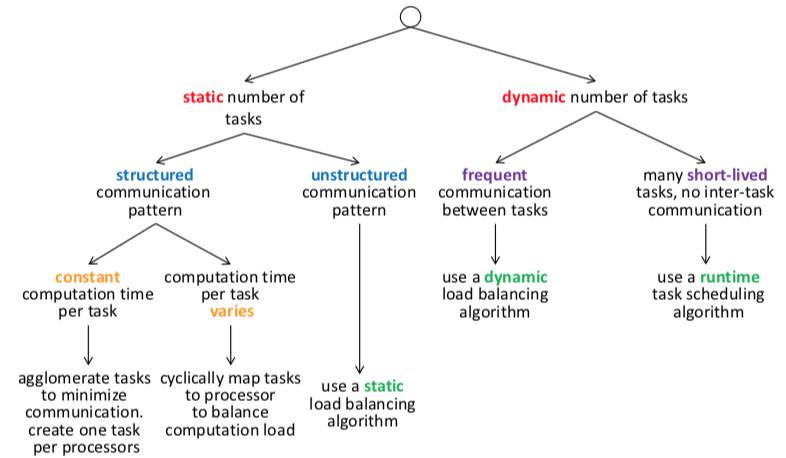
\includegraphics[width=\linewidth]{map}
  \end{tabularx}
  \begin{tabularx}{0.3\linewidth}{X}
    \textbf{Rules of thumb}: Finding optimal mapping in general is NP-hard (thus, must rely on heuristic), consider designs based on 1 task/processor and multiple tasks/processor, evaluate static \& dynamic alloc (dynamic -> ensure task allocator not a bottleneck, static -> ratio of tasks:processors at least 10:1)
  \end{tabularx}
  \section{Energy-efficient Computing and Data Centers}
  \subsubsection{ARM Cortex-A family Vs general purpose Intel/AMD x86 servers}
  \begin{tabularx}{\columnwidth}{X|X}
    \textbf{Similarities}       & \textbf{Differences} \\ \hline
    \begin{itemize}
      \item Processors cores + RAM + I/O interfaces + misc. peripherals
      \item Cores use similar exec model (pipelines)
      \item Memory hierarchy (L1 + L2 + RAM)
      \item Uses Virtual Memory
      \item Uses commodity Linux -- Supports all programming models available on Linux, most server SW is available, Porting is trivial
      \item Hardware virtualization, hardware-level security
    \end{itemize} &
    \begin{itemize}
      \item RISC Instruction-Set Architecture
      \item Heterogeneous cores (big.LITTLE) -- Fast cores / slow cores
      \item Lower instruction-level parallelism exploitation
      \item Smaller L1/L2 caches
      \item Less RAM (0.5 GB – 4GB), typically non-upgradable, depends on config
      \item Lower main-memory bandwidth
      \item Simpler I/O interfaces (USB2.0/USB 3.0/SATA2), next gen: PCI-Express, SATA 3
    \end{itemize}
  \end{tabularx}
  \subsection{Cloud Computing}
  \begin{itemize}
    \item Abstraction of underlying applications, information, content and resources, allows resources to be provided and consumed in a more elastic manner and on demand.
    \item Models: Software/Platform/Infrastructure as a Service (SaaS e.g. Google Apps; PaaS, e.g. Google App Engine; IaaS, e.g. Amazon EC2)
    \item Deployment models: Private, Community, Public, Hybrid Cloud
    \item Characteristics: On-demand self-service, Broad network access, Resource pooling, Rapid elasticity, Measured service
  \end{itemize}
  \subsection{Virtualisation}
  \begin{itemize}
    \item Creation of a virtual version of something. Access resource without being concerned with where and how the resource is physically located/managed.
    \item Types: \textbf{Services}, \textbf{Server}, \textbf{Storage}, \textbf{Network}
  \end{itemize}
\end{multicols*}
\end{document}
